\documentclass[a4paper,12pt]{article}

% Packages
\usepackage{graphicx}  % For images
\usepackage{amsmath}   % For math symbols
\usepackage{hyperref}  % For hyperlinks
\usepackage{fancyhdr}  % For headers
\usepackage{geometry}  % For page layout
\usepackage{xcolor}    % For colors
\usepackage{listings}  % For code snippets
\usepackage{float}     % For image positioning
\usepackage{caption}
\usepackage[utf8]{inputenc} % For special characters
\geometry{a4paper, margin=1in}

% Fancy header/footer settings
\pagestyle{fancy}
\fancyfoot[R]{\thepage} % Right-align page number in the footer
\fancyfoot[C]{}         % Clear the default center-aligned page number

% Title information
\title{Zephyr RTOS Project Report}
\author{
107474-Joseane Pereira \\
109050-Gabriel Costa \\
Universidade de Aveiro, DETI
}
\date{\today}

\begin{document}
\begin{figure}
    \centering
    
\includegraphics[width=0.3\linewidth]{ua.pdf}
    \label{fig:enter-label}
\end{figure}
\maketitle
\newpage
\tableofcontents
\newpage

\section{Introduction}
The aim of this project is to apply the Linux Real-Time Services and the Real-Time Model to the development of a real-life inspired real-time application. The project encompasses a set of cooperating tasks, involving synchronization, shared resources, access to a real-time database, etc.

\section{Architecture}
\subsection{System Overview}
In this project, the real-time monitoring system is structured around several primary tasks. These tasks were scheduled using a Static Table-Based Scheduler, which is the most important module of this project. 

Given our use-case, we also implemented a RTDB, in order to have a structure that could store the changes in information.

\subsection{Task}
We designed a structure named \textbf{Task} to encapsulate all the necessary information about a task. This includes attributes such as its period (measured in ticks), execution time, and other relevant details.

This information is then used in the STBS to store and manage the information of each task of the system.

\subsection{Static Table-Based Scheduler Implementation}
\subsubsection{Initialization}
To initialize our STBS, we define the time each micro-cycle has, the maximum number of tasks, initialize the number of tasks that the table currently has to 0, and finally, initialize a list of the "Tasks" of the system.

\subsubsection{STBS\_AddTask}
This function is only responsible for initializing a new "Task" and adding it to the STBS list of tasks, making sure it doesn't exceed the maximum number of tasks.

\subsubsection{STBS\_Start}
The function \textbf{STBS\_Start} is invoked after all tasks have been added to the scheduler. Its primary responsibility is to determine whether the tasks are schedulable and, if so, to handle their scheduling and execution. Specifically, this involves assigning each task to its respective micro-cycle. 

Once the scheduling is complete, the function iterates through the micro-cycles, resuming and executing all tasks within each cycle in the predefined order. This process continues until the program is stopped.

\subsubsection{STBS\_print\_content}
This function is responsible for displaying the contents of the scheduler table in a structured, table-like format.

\begin{figure}[H]
    \centering
    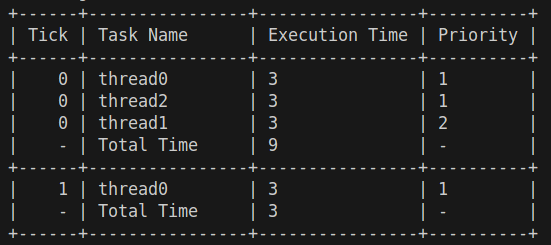
\includegraphics[width=0.91\linewidth]{STBS_table.png}
    \caption{Scheduler's table}
    \label{fig:scheduler_table}
\end{figure}

\subsubsection{STBS\_destroy}
This function is responsible for releasing the memory allocated for the STBS and the table it generated.

\subsection{Real-Time Database (RTDB)}
The RTDB is used to store the states of LEDs and buttons, ensuring synchronized access and updates by different tasks.

\section{Tasks}
\subsection{Task Characteristics}
The system is composed by the following tasks:
\begin{enumerate}
    \item \textbf{Task 0}: Updates the RTDB with the button states.
    \item \textbf{Task 1}: Updates the LED states based on the button states from the RTDB.
    \item \textbf{Task 2}: Validates RTDB entries and resets them if they are corrupted.
\end{enumerate}

Each task in the system is assigned a specific priority and a period to ensure timely execution and prevent task starvation. The following table outlines the task priorities and activation periods.


\subsection{Execution Patterns and Relevant Events}
The RTDB is critical for data synchronization:
\begin{itemize}
    \item \textbf{Task 0} is responsible for updating the RTDB with the current states of the buttons. It reads the states of the buttons and writes these states to the RTDB. This task runs periodically every 50ms with priority 1.
    \item \textbf{Task 1} is responsible for updating the LED states based on the button states stored in the RTDB. It reads the button states from the RTDB and updates the LED states accordingly. This task runs periodically every 100ms with priority 2.
    \item \textbf{Task 2} is responsible for validating the RTDB entries and resetting them if they are corrupted. It reads the states of the LEDs and buttons from the RTDB and checks for any invalid values. If any invalid values are found, it resets them to a default state. This task runs periodically every 100ms with priority 1.

    \item Since there aren't multiple tasks trying to write to the RTDB there is no need to implement mutexes or other mechanisms to handle concurrent access.
\end{itemize}


% \subsubsection{Inter-Task Communication}
The tasks communicate through the RTDB, which acts as a shared data structure. Task 0 writes the button states to the RTDB, and Tasks 1 and 2 read these states. Task 1 updates the LED states based on the button states, and Task 2 validates the RTDB entries. This communication pattern ensures that the tasks operate on the most recent data without conflicts.

\section{Real-Time System Characterization}
\subsection{System Performance}
To evaluate the system's performance, we analyzed both the task execution times and the scheduler's overhead.

Each task takes approximately 2 to 3 milliseconds to execute, depending on its complexity. The scheduler, when managing three tasks in a single micro-cycle, requires 8 to 9 milliseconds to complete. For cycles with only one task, the scheduler takes around 2 to 3 milliseconds. This demonstrates that the scheduler overhead is minimal, contributing only a few microseconds per task execution. Such low overhead indicates a highly efficient scheduler.

The measurements were obtained through the following modifications:
\begin{itemize} 
    \item In each task, the execution start and finish times were recorded using \textbf{k\_uptime\_get}. The difference between these timestamps was calculated and printed to determine the execution time of the task .
    \item In the scheduler, the start and finish times of each micro-cycle were recorded using the same function. The difference between these timestamps was printed to assess the scheduler's execution time.
\end{itemize}

These results confirm that the scheduler introduces negligible performance overhead, maintaining system responsiveness and ensuring real-time task scheduling efficiency.


\subsection{System Schedulability}
% To confirm that all tasks meet their deadlines, we perform a schedulability analysis using the \textbf{Least Upper Bound (LUB)} method.

% \textbf{Utilization Factor (U)}: Given that each task is independent and periodic, we can calculate the utilization factor \( U \) using:

% \[
% U = \sum_{i=1}^n \frac{C_i}{T_i}
% \]

% where \( C_i \) is the computation time and \( T_i \) is the period of each task. Assuming each task completes within its assigned period, this calculation helps ensure that the system remains schedulable.

% For the tasks in our system, the utilization factor is calculated as follows:

% \[
% U = \frac{3}{50} + \frac{3}{100} + \frac{3}{100} = 0.12 
% \]

Since our system uses a Static Table-Based Scheduler (STBS), we added code to verify if the task set is schedulable. This code checks whether any task is delayed beyond its deadline. Also, the only shared resource is the Real-Time Database (RTDB), and because no more than one task modifies its values at the same time, there is no need to account for resource conflicts.

Our system operates with a 50ms tick. Based on the resulting schedule table \ref{fig:scheduler_table}, we can confirm that the task set is indeed schedulable..


\section{Use-Case Implementation}
\subsection{Smart I/O Module}
Here, we implemented a mapping from each button to each led, meaning that each button will toggle the state of the respective led.

\subsection{UART Communication Protocol}
In order for the computer to communicate with the Microcontroller, we implemented a simple protocol. It consists of writing commands in the PC, and receiving an ACK message, confirming if the command was executed successfully or if something went wrong (e.g: command doesn't exist or wrong checksum).

% In our implementation, every time a command is completed (the user typed the character "\#") the command is processed and executed (if prompted correctly). The respective acknowledge is then sent back as a response.
For this project, we decided to process the command inside the UART interrupt function meaning that we assume that the overhead is close to 0, however, we understand that this is not the best practice, since it can add overhead to the execution of the tasks.

\section{Tests}
The tests for the scheduler verify that tasks are added correctly and meet their deadlines. 
% In other words, we verify if the scheduler can schedule a schedulable system and detects when the system is not schedulable.
The test suite includes the following.
\begin{itemize}
    \item \textbf{Scheduler Test}: Verifies that the scheduler can schedule a schedulable system and detects when the system is not schedulable.
    \item \textbf{Scheduler organization}: Verifies that tasks are ordered by their priority and by their period.
    % \item \textbf{Task Deadline Test}: Verifies that tasks meet their deadlines.
\end{itemize}

\subsection{Scheduler Test}
When testing the scheduler, we noticed that it wasn't detecting when the tasks exceeded their deadline, so we had to make some small changes (which are marked in the code with "CHANGED"), namely, adding this condition
\begin{figure}[H]
    \centering
    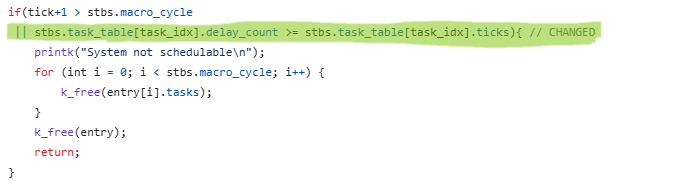
\includegraphics[width=0.91\linewidth]{code_change.png}
    % \caption{Code change}
    \label{fig:code_change}
\end{figure}

which checks if a task is delayed past it's deadline.

Now, for the tests, when creating the table, we tested if the tasks that executed in the same micro-cycle with the same priority, are ordered by their period, meaning that the ones with lower period execute first.
\begin{figure}[H]
    \centering
    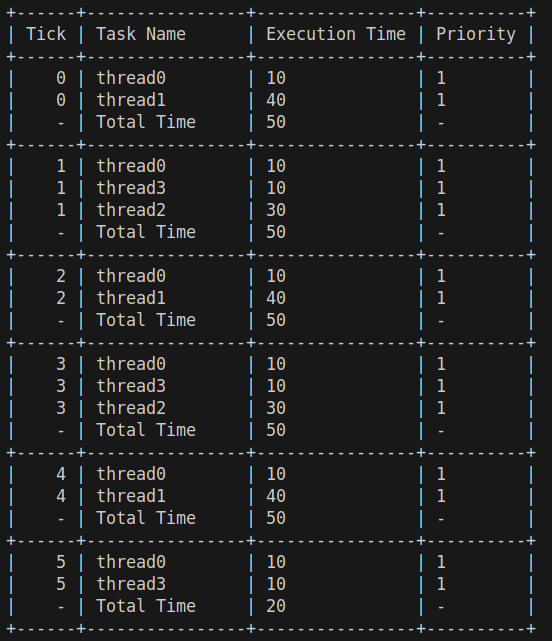
\includegraphics[width=0.6\linewidth]{STBS_test_period.png}
    % \caption{Code change}
    \label{fig:STBS_test_period}
\end{figure}

Then, we tested whether tasks with higher priority execute first.
\begin{figure}[H]
    \centering
    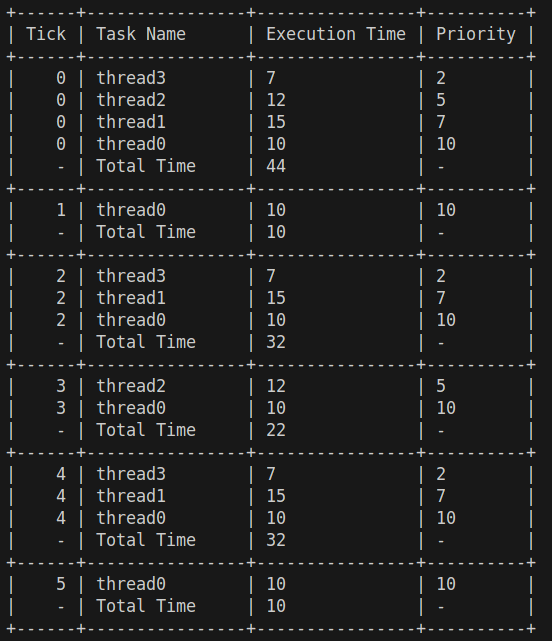
\includegraphics[width=0.6\linewidth]{STBS_test_priority.png}
    % \caption{Code change}
    \label{fig:STBS_test_priority}
\end{figure}

Last but not least, we needed to test if the our code could recognize if a system is not schedulable. For that we did the following tests:
\begin{itemize}
    \item We created a table with a micro-cycle of 50 ms and 4 tasks. These tasks had a period of 1, 3, 2, 2 ticks, priorities of 10, 5, 7, 2 and 20, 25, 30, 15 ms of execution time, respectively. Since the first task has a period of 1 tick and had the lowest priority, it was not able to meet its first deadline, which makes this system not schedulable.

    \item For the next test, we changed the priority of the first task to 1. This system is also not schedulable since the third task is not able to execute before it meets it's deadline, since in the first tick it executes the first and fourth task, and in the second one it executes the first and the second, leaving no time for the third task to execute.
\end{itemize}

\section{Results}
The results of our tests confirm that the scheduler is functioning as intended. Tasks are correctly initialized, added, and executed. Furthermore, all tasks meet their deadlines within the specified margins when the system is schedulable. Non-schedulable systems are accurately identified, validating the robustness of our scheduler.

\section{Conclusion}
In this project, a multi-threaded system was successfully implemented to manage tasks in a real-time environment. The scheduler ensures that tasks are executed periodically and meet their deadlines. The RTDB provides synchronized access to shared data, preventing data corruption. Overall, the project demonstrates effective use of periodic task scheduling, synchronization, and real-time data management.

\section{Appendice}
We made a change in the code regarding the use of checksums. Before, we didn't send the checksum correctly to the microcontroller. We were calculating the checksum when we had a complete frame and we would send it to the function who executes the command. To fix this, we made the following changes:
\begin{figure}[H]
    \centering
    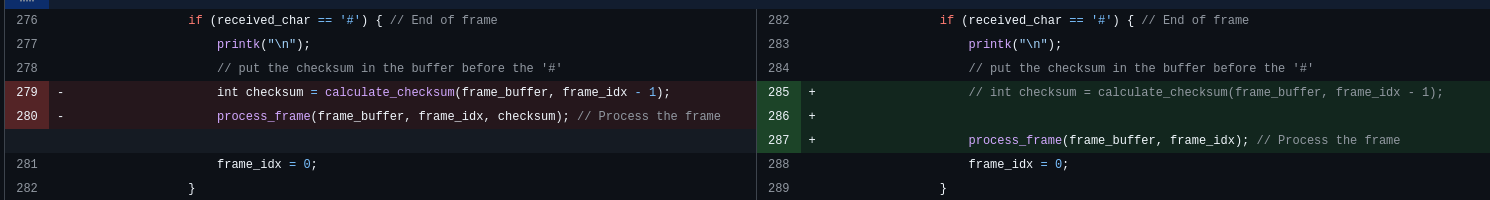
\includegraphics[width=1\linewidth]{checksum_change.png}
    \caption{Receiving checksum as an input instead of calculating it}
    \label{fig:checksum_change}
\end{figure}

\begin{figure}[H]
    \centering
    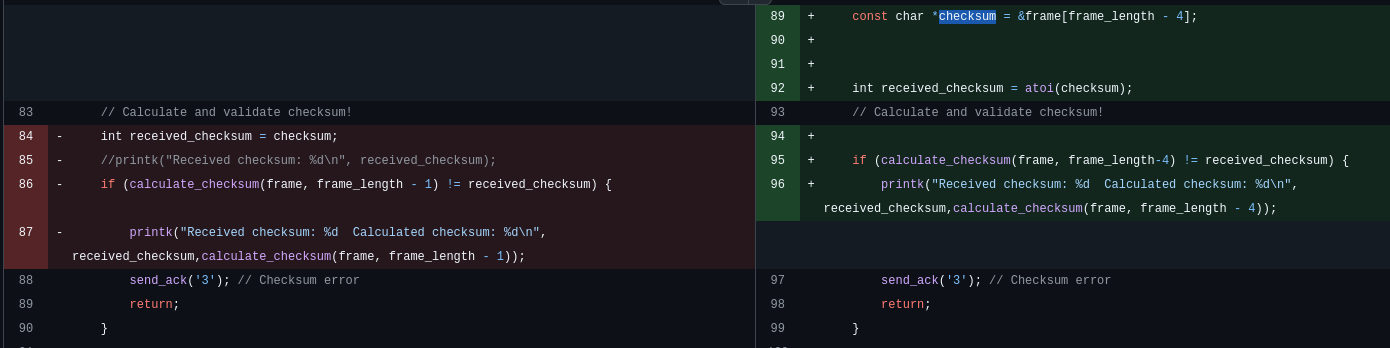
\includegraphics[width=1\linewidth]{checksum_change1.png}
    \caption{Compare the checksum calculated to the one received as an input}
    \label{fig:checksum_change1}
\end{figure}

\end{document}